\documentclass[conference, 14pt]{IEEEtran}
\IEEEoverridecommandlockouts
\usepackage{blindtext}
\usepackage{graphicx}
\graphicspath{ {./images/}  }

\begin{document}

\title{ECSE 331\\
    Laboratory No. 1\\
    Introduction to PSPICE\\
    \Large \today\\
}

\author
{
    \IEEEauthorblockN{Seyed Yazdan Zinati}
    \IEEEauthorblockA{260928077 \\
    \textit{seyed.zinati@mail.mcgill.ca}}

    \and

    \IEEEauthorblockN{James Wu}
    \IEEEauthorblockA{260929944 \\
    \textit{james.wu4@mail.mcgill.ca}}
}


\maketitle

\clearpage

\begin{abstract}
    SPICE (Simulation Program for Integrated Circuits Emphasis) is a general-purpose circuit simulator. In this laboratory, we demonstrate the basics of PSPICE using three experiments. The results obtained using PSPICE simulations are then compared with theoretical results obtained by manual circuit analysis. The three experiments consist of finding the voltage at given nodes, the current in given branches, and the Thevenin and Norton equivalent in three circuits. Despite finding the same results using manual circuit analysis, analysis using PSPICE simulation is significantly faster and removes the possibility of calculation errors. Moreover, PSPICE enables us to solve complicated circuits, which would be a very long task if done manually.
\end{abstract}


\section{Introduction}

\subsection*{Experiment 1}
This experiment required using PSPICE to find the voltage values at the three nodes (1, 2, and 3) in the given circuit. The given circuit is shown in figure \ref{fig:circuit1}.
\begin{figure}[h]
    \caption{Exercise circuit}
    \centering
    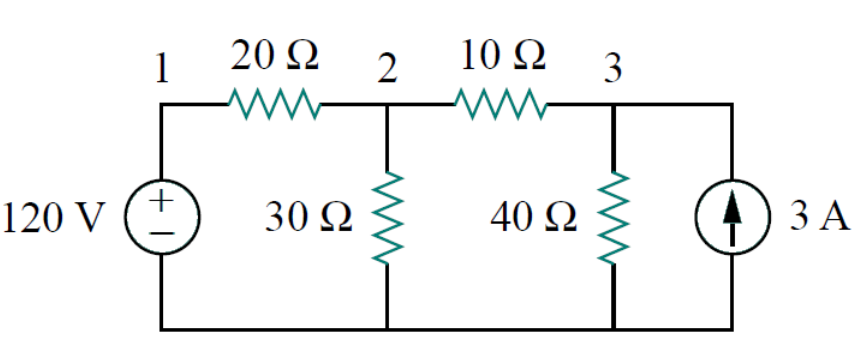
\includegraphics[scale=0.30]{ex1}
    \label{fig:circuit1}
\end{figure}

\subsection*{Experiment 2}
This experiment required using PSPICE to find the current values in three branches ($i_1$, $i_2$, and $i_3$). The given circuit is shown in figure \ref{fig:circuit2}.
\begin{figure}[h]
    \caption{Exercise circuit}
    \centering
    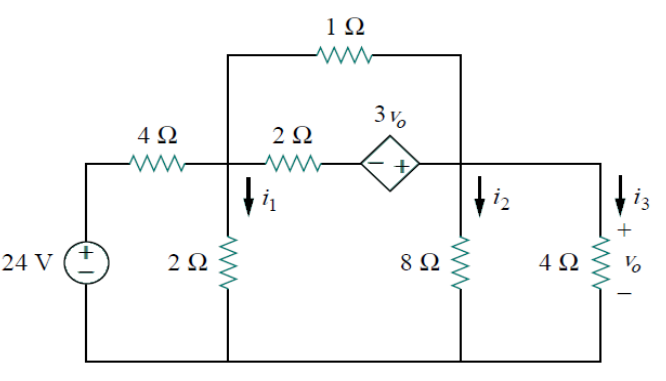
\includegraphics[scale=0.39]{ex2}
    \label{fig:circuit2}
\end{figure}

\subsection*{Experiment 3}
This experiment required using PSPICE to find the Thevenin/Norton equivalent of a given circuit. The given circuit is shown in figure \ref{fig:circuit3}.
\begin{figure}[h]
    \caption{Exercise circuit}
    \centering
    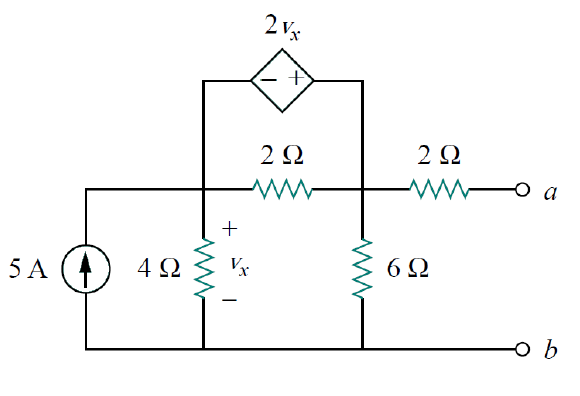
\includegraphics[scale=0.39]{ex3}
    \label{fig:circuit3}

\end{figure}
\section{Exercises}

\subsection{Exercise 1}
\blindtext

\subsection{Exercise 2}
\blindtext

\subsection{Exercise 3}
\blindtext

\section{Conclusion}
\blindtext

\end{document}
